\documentclass[expologarit]{subfiles}
\begin{document}

 \begin{center}
 \color{violet} \kml លំហាត់ទី៩
 \end{center}
គេមានអនុគមន៍ $f$ មួយកំណត់ដោយ $y=f(x)=\frac{x^2-4x+3}{x^2-3x+2}$ មានក្រាបតំណាង$(C)$។
\begin{enumerate}[k]
\item ចូររកដែនកំណត់នៃអនុគមន៍$f$។
\item គណនា $\lim_{x\to 2}f(x);\ \lim_{x\to \pm\infty}f(x)$ ។ រួចទាញរកសមីការអាស៊ីមតូតទាំងអស់ដែលមាន។
\item សិក្សាអថិរភាព និងសង់តារាងអថិរភាពនៃអនុគមន៍$f$។
\item ចូរសង់ក្រាប$(C)$ ក្នុងតម្រុយ $\left(O,\overrightarrow{i},\overrightarrow{j}\right)$។
\end{enumerate}
\begin{center}
\color{violet} \kml ដំណោះស្រាយ
\end{center}
\begin{enumerate}[k]
\item រកដែនកំណត់នៃអនុគមន៍$f$\\[0.25cm]
យើងមាន $y=f(x)=\frac{x^2-4x+3}{x^2-3x+2}=\frac{(x-1)(x-3)}{(x-1)(x-2)}=\frac{x-3}{x-2}$\\[0.25cm]
$f(x)$ មានន័យលុះត្រាតែ $x-2 \neq 0 \Leftrightarrow\quad  x\neq 2$\\[0.25cm]
ដូចនេះ \fbox{$D_f=\mathbb{R}-\{2\}$}
\item គណនា $ \lim_{x\to 2}f(x);\ \lim_{x\to \pm\infty}f(x) $ 
\begin{flalign*}
&\lim_{x\to 2}f(x)=\lim_{x\to 2}\frac{x^2-4x+3}{x^2-3x+2}=\pm\infty &\\
&\lim_{x\to \pm\infty}f(x)=\lim_{x\to \pm\infty}\frac{x^2-4x+3}{x^2-3x+2}=\lim_{x\to \pm\infty}\frac{x^2\left(1-\frac{4}{x}+\frac{3}{x^2}\right)}{x^2\left(1-\frac{3}{x}+\frac{2}{x^2}\right)}=1
\end{flalign*}
 ទាញរកសមីការអាស៊ីមតូតទាំងអស់ដែលមាន\\
 ដោយ $ \lim_{x\to 2}f(x)=\pm\infty$\\[0.25cm]
  ដូចនេះ \fbox{បន្ទាត់  $x=2$ ជាអាស៊ីមតូតឈរនៃក្រាប$(C)$}
  \\[0.25cm]
  ដោយ $\lim_{x\to \pm\infty}f(x)=1$\quad  ដូចនេះ \fbox{បន្ទាត់ $y=1$ ជាអាស៊ីមតូតដេកនៃក្រាប$(C)$}
  \newpage 
\item សិក្សាអថិរភាព និងសង់តារាងអថិរភាពនៃអនុគមន៍$f$
\\
ដេរីវេ
\begin{flalign*}
f'(x)=\left(\frac{x-3}{x-2}\right)'&=\frac{(x-3)'\left(x-2\right)-\left(x-2\right)'\left(x-3\right)}{\left(x-2\right)^2}&\\
&=\frac{1}{(x-2)^2} \ >0\quad \forall x\in D_f
\end{flalign*}
តារាងសញ្ញា $f'(x)$
\\[0.2cm]
\begin{tikzpicture}[scale=0.5]
   \tkzTabInit{$x$ / 1.5 , $f'(x)$ / 2}{$\ \ -\infty$ ,$2$, $+\infty\ \ $}
   \tkzTabLine{,+, d,+, }
\end{tikzpicture}
\begin{itemize}
\item $f'(x)>0$ ពេល $x\in\left(-\infty ,2\right)\cup\left(2,+\infty\right)\Rightarrow $ អនុគមន៍ $f$ កើន ពេល  $x\in\left(-\infty ,2\right)\cup\left(2,+\infty\right) $
\end{itemize}
តារាងអថេរភាពនៃ $f$\\[0.2cm]
\begin{tikzpicture}
   \tkzTabInit[lw=1,lgt=1,espcl=1.5]{$x$ / 0.75 , $f'(x)$ / 1, $f(x)$/2}{$ -\infty$ , $2$, $+\infty  $}
   \tkzTabLine{,  +, d,+ ,}
   \tkzTabVar{-/ $1$,   +D-/$+\infty$/$-\infty$, +/ $1$}
\end{tikzpicture}
\item សង់ក្រាប$(C)$ ក្នុងតម្រុយ $\left(O,\overrightarrow{i},\overrightarrow{j}\right)$
\begin{flalign*}
(C)\cap (x'ox)\Leftrightarrow y=0\quad\Leftrightarrow\quad & x-3=0 &\\
												\Rightarrow\quad & x=3
\end{flalign*}
\begin{flalign*}
(C)\cap (y'oy)\Leftrightarrow x=0\quad\Rightarrow y=\frac{0^2-4(0)+3}{0^2-3(0)+2}=\frac{3}{2}&&
\end{flalign*}
\end{enumerate}


 \begin{center}
\begin{tikzpicture}[x=1cm,y=1cm]
\begin{axis}[scale=1,
          xmax=8.5,ymax=7.5,
          axis lines=middle,
          xmin=-3.5,ymin=-7.5,          
          xtick={-11,-10,...,10},
          ytick={-11,-10,...,12}  ,
          xlabel=$x$   ,
          ylabel=$y$   ,x=1cm, y=1cm
          ] 
\addplot[domain=-13:13 ,restrict y to domain=-14:14,line width=1pt,samples=1000,smooth,name path=A,color=red] {(x^2-4*x+3)/(x^2-3*x+2)};
\addplot[domain=-14.5:13,samples=100,smooth,line width=1.5pt ] {1}node[sloped, near end,above]{$\qquad\qquad\qquad\qquad\qquad
y=1$};

%\addplot [color=black]coordinates {(-2.5,0)} node[below ]{$x'$};

%\node at(0,-1){$\bullet$};

%\draw[dashed](1,0)--(1,1)--(0,1);

             %\addplot[gray, pattern=north west lines] fill between[of=A and B, soft clip={domain=1:2}];
           
              \draw (0,0)rectangle (0.2,0.2);
           
             \draw[line width=1.5pt] (2,-14)--(2,14)node[sloped, near end,below]{$x=2$};
                          
            \draw (2.5,-7) node {$(C)$};

              \draw (0,1.5) node {$\bullet$};
              \draw (3,0) node {$\bullet$};

\end{axis}
\end{tikzpicture}
 \end{center}
\end{document}